\documentclass[uplatex,a4j,11pt,dvipdfmx]{jsarticle}
\bibliographystyle{junsrt}

\usepackage{listings,jvlisting}
\usepackage{url}
\usepackage{graphicx}
\usepackage{gnuplot-lua-tikz}
\usepackage{pgfplots}
\usepackage{tikz}
\usepackage{amsmath,amsfonts,amssymb}
\usepackage{bm}
\usepackage{siunitx}
\usepackage{braket}
\usepackage{autobreak}

\definecolor{OliveGreen}{rgb}{0.0,0.6,0.0}
\definecolor{Orenge}{rgb}{0.89,0.55,0}
\definecolor{SkyBlue}{rgb}{0.28, 0.28, 0.95}
\lstset{
  language={verilog}, % 言語の指定
  basicstyle={\ttfamily},
  identifierstyle={\small},
  commentstyle={\smallitshape},
  keywordstyle={\small\bfseries},
  ndkeywordstyle={\small},
  stringstyle={\small\ttfamily},
  frame={tb},
  breaklines=true,
  columns=[l]{fullflexible},
  xrightmargin=0zw,
  xleftmargin=3zw,
  lineskip=-0.5ex,
  keywordstyle={\color{SkyBlue}},     %キーワード(int, ifなど)の書体指定
  commentstyle={\color{OliveGreen}},  %注釈の書体
  stringstyle=\color{Orenge}          %文字列
}
\pagestyle{empty}
\makeatletter
\def\fgcaption{\def\@captype{figure}\caption}
\makeatother

\makeatletter
\def\fgcaption{\def\@captype{figure}\caption}
\makeatother
\newcommand{\setsections}[3]{
\setcounter{section}{#1}
\setcounter{subsection}{#2}
\setcounter{subsubsection}{#3}
}
\newcommand{\mfig}[3][width=15cm]{
\begin{center}
\includegraphics[#1]{#2}
\fgcaption{#3 \label{fig:#2}}
\end{center}
}
\newcommand{\gnu}[2]{
\begin{figure}[hptb]
\begin{center}
\input{#2}
\caption{#1}
\label{fig:#2}
\end{center}
\end{figure}
}
\newcommand{\up}{\uparrow}
\newcommand{\dn}{\downarrow}


\usepackage{amsmath}
\makeatletter
%%%
%%%  左側、右側に subscript を付記する。
%%%  使い方: \subscripts{左下}{中身}{右下}
%%%
%%%  by FUJIWARA Hiroshi <fujiwara (at) acs.i.kyoto-u.ac.jp>
%%%
\newcommand{\subscripts}[3]{%
  \@mathmeasure\z@\displaystyle{#2}%
  \global\setbox\@ne\vbox to\ht\z@{}\dp\@ne\dp\z@
  \setbox\tw@\box\@ne
  \@mathmeasure4\displaystyle{\copy\tw@_{#1}}%
  \@mathmeasure6\displaystyle{{#2}_{#3}}%
  \dimen@-\wd6 \advance\dimen@\wd4 \advance\dimen@\wd\z@
  \hbox to\dimen@{}\mathop{\kern-\dimen@\box4\box6}%
}
\makeatother

\everymath{\displaystyle}
\begin{document}
\title{統計物理学 No.3}
\author{82311971 佐々木良輔}
\date{}
\maketitle
\subsection*{[1] (a)}
$h=0$とすると$m$の3次で展開した自己無撞着方程式は
\begin{align}
    m=\frac{T_c}{T}m-\frac{1}{\mu_s}^2\left(\frac{T_c}{T}\right)^3m^3
\end{align}
$T<T_c$で$m\neq0$より,両辺を$m$で割ると
\begin{align}
  \begin{array}{cc}
    &1=\frac{T_c}{T}-\frac{1}{\mu_s}^2\left(\frac{T_c}{T}\right)^3m^2\\
    \iff&0=\left(\frac{T_c}{T}-1\right)-\frac{1}{\mu_s}^2\left(\frac{T_c}{T}\right)^3m^2\\
    \iff&m=\pm\mu_s\frac{T}{T_c}\sqrt{\frac{T_c-T}{T_c}}
  \end{array}
\end{align}
となる.
\subsection*{(b)}
自己無撞着方程式の両辺を$h$で微分すると
\begin{align}
  \chi=\frac{T_c}{T}\left(\chi+\frac{1}{zJ}\right)-\frac{1}{\mu_s^2}\left(\frac{T_c}{T}\right)^33\left(m+\frac{h}{zJ}\right)^2\left(\chi+\frac{1}{zJ}\right)
\end{align}
ただし$\chi=\partial m/\partial h$である.
\subsubsection*{$T>T_c$のとき}
$T>T_c$では$m=0$である.また(3)式において$h\rightarrow0$とすれば
\begin{align}
  \begin{array}{cc}
    &\chi_0=\frac{T_c}{T}\left(\chi+\frac{1}{zJ}\right)\\
    \iff&\chi_0=\frac{\frac{T_c}{T}\frac{1}{zJ}}{1-\frac{T_c}{T}}=\frac{T_c}{zJ(T-T_c)}
  \end{array}
\end{align}
となる.
\subsubsection*{$T<T_c$のとき}
(3)式より
\begin{align}
  \begin{array}{cc}
    &\chi\left(1-\frac{T_c}{T}+\frac{3}{\mu_s^2}\left(\frac{T_c}{T}\right)^3\left(m+\frac{h}{zJ}\right)^2\right)=\frac{1}{zJ}\left(\frac{T_c}{T}-\frac{3}{\mu_s^2}\left(\frac{T_c}{T}\right)^3\left(m+\frac{h}{zJ}\right)^2\right)\\
    \iff&\chi=\frac{\frac{1}{zJ}\left(\frac{T_c}{T}-\frac{3}{\mu_s^2}\left(\frac{T_c}{T}\right)^3\left(m+\frac{h}{zJ}\right)^2\right)}{1-\frac{T_c}{T}+\frac{3}{\mu_s^2}\left(\frac{T_c}{T}\right)^3\left(m+\frac{h}{zJ}\right)^2}
  \end{array}
\end{align}
ここで$h\rightarrow0$とすると
\begin{align}
  \chi_0=\frac{\frac{1}{zJ}\left(\frac{T_c}{T}-\frac{3}{\mu_s^2}\left(\frac{T_c}{T}\right)^3m^2\right)}{1-\frac{T_c}{T}+\frac{3}{\mu_s^2}\left(\frac{T_c}{T}\right)^3m^2}
\end{align}
さらに$T\simeq T_c$から$m$として(2)式の結果を用いると
\begin{align}
  \begin{split}
    \frac{1}{\mu_s^2}\left(\frac{T_c}{T}\right)^3m^2&=\frac{1}{\mu_s^2}\left(\frac{T_c}{T}\right)^3\mu_s^2\left(\frac{T}{T_c}\right)^3\left(\frac{T_c}{T}-1\right)\\
    &=\frac{T_c}{T}-1
  \end{split}
\end{align}
なので(6)式は
\begin{align}
  \begin{split}
    \chi_0&=\frac{\frac{1}{zJ}\left(\frac{T_c}{T}-3\left(\frac{T_c}{T}-1\right)\right)}{1-\frac{T_c}{T}+3\left(\frac{T_c}{T}-1\right)}\\
    &=-\frac{(3T-2T_c)}{2zJ(T-T_c)}
  \end{split}
\end{align}
となる.図1に$zJ=1$, $T_c=5$としたときの$\chi_0$の片対数グラフを示す.
赤線と青線はそれぞれ$T>T_c$, $T<T_c$の場合である.図から$T\simeq T_c$では挙動$T>T_c$, $T<T_c$が近い挙動を取ることがわかる.
\begin{center}
  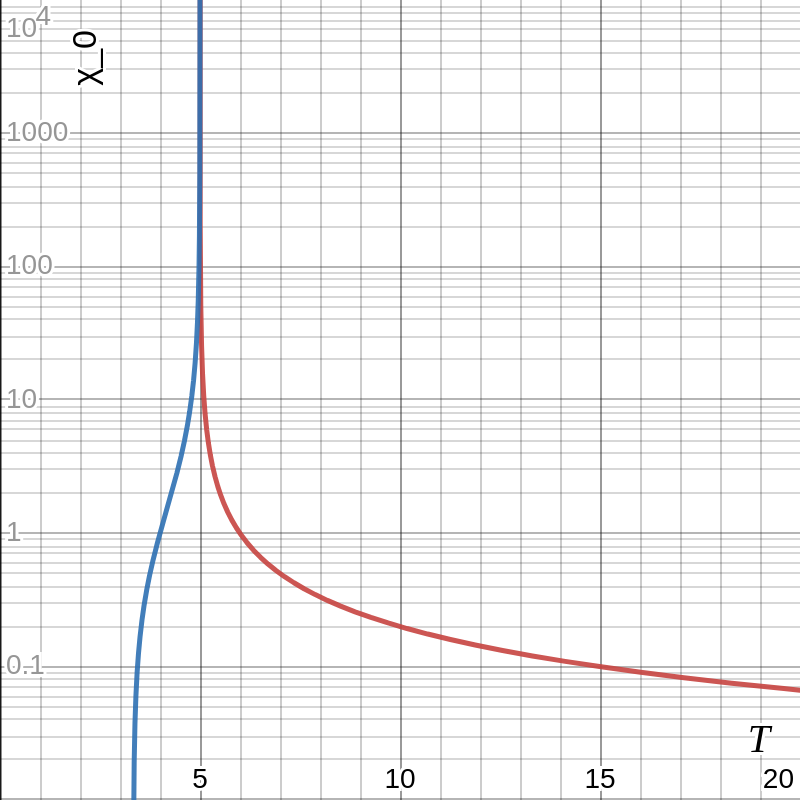
\includegraphics[width=6cm]{xi_0.png}
  \fgcaption{$zJ=1$, $T_c=5$としたときの$\xi_0$. 赤線は$T>T_c$, 青線は$T<T_c$の場合.}
\end{center}
\subsection*{[2] (a)}
$S^+$の期待値は
\begin{align}
  \begin{split}
    \langle S^+\rangle&=
    \left(\cos\frac{\theta}{2}\Bra{\up}+e^{-i\phi}\sin\frac{\theta}{2}\Bra{\dn}\right)\Ket{\up}\Bra{\dn}
    \left(\cos\frac{\theta}{2}\Ket{\up}+e^{i\phi}\sin\frac{\theta}{2}\Ket{\dn}\right)\\&=
    \left(\cos\frac{\theta}{2}\times1+e^{-i\phi}\sin\frac{\theta}{2}\times0\right)
    \left(\cos\frac{\theta}{2}\times0+e^{i\phi}\sin\frac{\theta}{2}\times1\right)\\&=
    e^{i\phi}\cos\frac{\theta}{2}\sin\frac{\theta}{2}=\frac{e^{i\phi}}{2}\sin\theta
  \end{split}
\end{align}
同様にして$S^-$の期待値は
\begin{align}
  \begin{split}
    \langle S^-\rangle&=
    \left(\cos\frac{\theta}{2}\Bra{\up}+e^{-i\phi}\sin\frac{\theta}{2}\Bra{\dn}\right)\Ket{\dn}\Bra{\up}
    \left(\cos\frac{\theta}{2}\Ket{\up}+e^{i\phi}\sin\frac{\theta}{2}\Ket{\dn}\right)\\&=
    \left(\cos\frac{\theta}{2}\times0+e^{-i\phi}\sin\frac{\theta}{2}\times1\right)
    \left(\cos\frac{\theta}{2}\times1+e^{i\phi}\sin\frac{\theta}{2}\times0\right)\\&=
    k
  \end{split}
\end{align}
また$S^z$の期待値は
\begin{align}
  \begin{split}
    \langle S^z\rangle&=
    \left(\cos\frac{\theta}{2}\Bra{\up}+e^{-i\phi}\sin\frac{\theta}{2}\Bra{\dn}\right)\frac{1}{2}\left(\Ket{\up}\Bra{\up}-\Ket{\dn}\Bra{\dn}\right)
    \left(\cos\frac{\theta}{2}\Ket{\up}+e^{i\phi}\sin\frac{\theta}{2}\Ket{\dn}\right)\\&=
    \left(\cos\frac{\theta}{2}\Bra{\up}+e^{-i\phi}\sin\frac{\theta}{2}\Bra{\dn}\right)\frac{1}{2}
    \left(\cos\frac{\theta}{2}\Ket{\up}-e^{i\phi}\sin\frac{\theta}{2}\Ket{\dn}\right)\\&=
    \frac{1}{2}\left(\cos^2\frac{\theta}{2}-\sin^2\frac{\theta}{2}\right)=\frac{1}{2}\cos\theta
  \end{split}
\end{align}
である.
\subsection*{(b)}
XXZ鎖のハミルトニアンは$S^+$, $S^-$を用いて
\begin{align}
  H=\frac{J}{2}\sum_{j=1}^N\left(S_j^+S_{j+1}^-+S_j^-S_{j+1}^+\right)+J\Delta\sum_{j=1}^NS_j^zS_{j+1}^z-h\sum_{j=1}^NS_j^z
\end{align}
である.また傾けられた反強磁性状態は
\begin{align}
  \Ket{\Psi(\theta)}=\otimes_j\Ket{\psi(\theta,\psi_j)}=\Ket{\psi(\theta,0)}_1\otimes\Ket{\psi(\theta,\pi)}_2\otimes\cdots\otimes\Ket{\psi(\theta,\pi)}_N
\end{align}
と表される.
このときのエネルギー期待値は
\begin{align}
  \langle H\rangle=\Bra{\Psi}\frac{J}{2}\sum_{j=1}^N\left(S_j^+S_{j+1}^-+S_j^-S_{j+1}^+\right)\Ket{\Psi}+
  \Bra{\Psi}J\Delta\sum_{j=1}^NS_j^zS_{j+1}^z\Ket{\Psi}-
  \Bra{\Psi}h\sum_{j=1}^NS_j^z\Ket{\Psi}
\end{align}
である.ここで$S_j^+S_{j+1}^-$の期待値は
\begin{align}
  \begin{split}
    \Bra{\Psi}S_j^+S_{j+1}^-\Ket{\Psi}=&
    \subscripts{N}{\Bra{\psi(\theta,\pi)}}{}
    \otimes\cdots\otimes
    \subscripts{j+1}{\Bra{\psi(\theta,\phi_{j+1})}}{}\otimes
    \subscripts{j}{\Bra{\psi(\theta,\phi_j)}}{}
    \otimes\cdots\otimes
    \subscripts{1}{\Bra{\psi(\theta,0)}}{}
    S_j^+S_{j+1}^-\\
    &\Ket{\psi(\theta,0)}_1\otimes\cdots\otimes
    \Ket{\psi(\theta,\phi_j)}_j\otimes
    \Ket{\psi(\theta,\phi_{j+1})}_{j+1}\otimes\cdots\otimes\Ket{\psi(\theta,\pi)}_N\\
    =&\subscripts{1}{\Braket{\psi(\theta,0)|\psi(\theta,0)}}{1}\times\cdots\times
    \subscripts{j}{\Braket{\psi(\theta,\phi_j)|S_j^+|\psi(\theta,\phi_j)}}{j}\times\\
    &\subscripts{j+1}{\Braket{\psi(\theta,\phi_{j+1})|S_{j+1}^-|\psi(\theta,\phi_{j+1})}}{j+1}
    \times\cdots\times\subscripts{N}{\Braket{\psi(\theta,\pi)|\psi(\theta,\pi)}}{N}\\
    =&\frac{e^{i\phi_j}}{2}\sin\theta\times\frac{e^{-i\phi_{j+1}}}{2}\sin\theta
  \end{split}
\end{align}
ただし$\phi_j$と$\phi_{j+1}$は必ずどちらかが$\pi$, もう片方が$0$になるので
\begin{align}
  \Bra{\Psi}S_j^+S_{j+1}^-\Ket{\Psi}=&-\frac{1}{4}\sin^2\theta
\end{align}
同様にして$S_j^-S_{j+1}^+$の期待値も
\begin{align}
  \Bra{\Psi}S_j^-S_{j+1}^+\Ket{\Psi}=&-\frac{1}{4}\sin^2\theta
\end{align}
したがって(14)式の右辺第1項は
\begin{align}
  \begin{split}
    \Bra{\Psi}\frac{J}{2}\sum_{j=1}^N\left(S_j^+S_{j+1}^-+S_j^-S_{j+1}^+\right)\Ket{\Psi}=&
    \frac{J}{2}\sum_{j=1}^N\Bra{\Psi}\left(S_j^+S_{j+1}^-+S_j^-S_{j+1}^+\right)\Ket{\Psi}\\
    =&-\frac{JN}{4}\sin^2\theta
  \end{split}
\end{align}
となる.次に$S_j^zS_{j+1}^z$の期待値は
\begin{align}
  \begin{split}
    \Braket{\Psi|S_j^zS_{j+1}^z|\Psi}=&
    \subscripts{N}{\Bra{\psi(\theta,\pi)}}{}
    \otimes\cdots\otimes
    \subscripts{j+1}{\Bra{\psi(\theta,\phi_{j+1})}}{}\otimes
    \subscripts{j}{\Bra{\psi(\theta,\phi_j)}}{}
    \otimes\cdots\otimes
    \subscripts{1}{\Bra{\psi(\theta,0)}}{}
    S_j^zS_{j+1}^z\\
    &\Ket{\psi(\theta,0)}_1\otimes\cdots\otimes
    \Ket{\psi(\theta,\phi_j)}_j\otimes
    \Ket{\psi(\theta,\phi_{j+1})}_{j+1}\otimes\cdots\otimes\Ket{\psi(\theta,\pi)}_N\\
    =&\subscripts{1}{\Braket{\psi(\theta,0)|\psi(\theta,0)}}{1}\times\cdots\times
    \subscripts{j}{\Braket{\psi(\theta,\phi_j)|S_j^z|\psi(\theta,\phi_j)}}{j}\times\\
    &\subscripts{j+1}{\Braket{\psi(\theta,\phi_{j+1})|S_{j+1}^z|\psi(\theta,\phi_{j+1})}}{j+1}
    \times\cdots\times\subscripts{N}{\Braket{\psi(\theta,\pi)|\psi(\theta,\pi)}}{N}\\
    =&\frac{1}{2}\cos\theta\times\frac{1}{2}\cos\theta=\frac{1}{4}\cos^2\theta
  \end{split}
\end{align}
したがって(14)式の右辺第2項は
\begin{align}
  \Bra{\Psi}J\Delta\sum_{j=1}^NS_j^zS_{j+1}^z\Ket{\Psi}=\frac{J\Delta N}{4}\cos^2\theta
\end{align}
次に$S_j^z$の期待値は
\begin{align}
  \begin{split}
    \Braket{\Psi|S_j^z|\Psi}=&
    \subscripts{N}{\Bra{\psi(\theta,\pi)}}{}
    \otimes\cdots\otimes
    \subscripts{j}{\Bra{\psi(\theta,\phi_j)}}{}
    \otimes\cdots\otimes
    \subscripts{1}{\Bra{\psi(\theta,0)}}{}
    S_j^z\\
    &\Ket{\psi(\theta,0)}_1\otimes\cdots\otimes
    \Ket{\psi(\theta,\phi_j)}_j\otimes\cdots\otimes\Ket{\psi(\theta,\pi)}_N\\
    =&\subscripts{1}{\Braket{\psi(\theta,0)|\psi(\theta,0)}}{1}\times\cdots\times
    \subscripts{j}{\Braket{\psi(\theta,\phi_j)|S_j^z|\psi(\theta,\phi_j)}}{j}
    \times\cdots\times\subscripts{N}{\Braket{\psi(\theta,\pi)|\psi(\theta,\pi)}}{N}\\
    =&\frac{1}{2}\cos\theta
  \end{split}
\end{align}
したがって(14)式の右辺第3項は
\begin{align}
  \Bra{\Psi}h\sum_{j=1}^NS_j^z\Ket{\Psi}=\frac{hN}{2}\cos\theta
\end{align}
となる.以上から(14)式は
\begin{align}
  \langle H\rangle=-\frac{JN}{4}\sin^2\theta+\frac{J\Delta N}{4}\cos^2\theta-\frac{hN}{2}\cos\theta
\end{align}
であり,したがって1スピンあたりのエネルギー期待値は
\begin{align}
  e(h,\theta)=\frac{\langle H\rangle}{N}=-\frac{J}{4}\sin^2\theta+\frac{J\Delta}{4}\cos^2\theta-\frac{h}{2}\cos\theta
\end{align}
となる.
\subsection*{(c)}
(24)式が極値を取るべきなので
\begin{align}
  \begin{split}
    \frac{\partial e}{\partial\theta}&=-\frac{J}{2}\sin\theta\cos\theta-\frac{J\Delta}{2}\sin\theta\cos\theta+\frac{h}{2}\sin\theta\\
    &=\frac{1}{2}\sin\theta\left(h-J(1+\Delta)\cos\theta\right)=0\\
    \therefore\qquad&\theta=0,\ \pi,\ \arccos\left(\frac{h}{J(1+\Delta)}\right) 
  \end{split}
\end{align}
\subsubsection*{$h>J(1+\Delta)$のとき}
このとき$\arccos(h/J(1+\Delta))$は定義域外であり,値を持たない.したがって極値は$\theta=0,\ \pi$である.それぞれでのエネルギー期待値は
\begin{align}
  \begin{split}
    e(h,0)=\frac{J\Delta}{4}-\frac{h}{2}\\
    e(h,\pi)=\frac{J\Delta}{4}+\frac{h}{2}
  \end{split}
\end{align}
であり$h\geq 0$から常に$e(h,0)$が小さい.したがって$h>J(1+\Delta)$では
\begin{align}
  \begin{split}
    \theta_0=0\\
    e_0(h)=\frac{J\Delta}{4}-\frac{h}{2}
  \end{split}
\end{align}
となる.
\subsubsection*{$h\leq J(1+\Delta)$のとき}
このとき極値は$\theta=0,\ \pi,\ \arccos(h/J(1+\Delta))$である.以下では$\theta'=\arccos(h/J(1+\Delta))$とする.
エネルギー期待値の2階微分は
\begin{align}
  \begin{split}
    \frac{\partial^2 e}{\partial\theta^2}&=\frac{\partial}{\partial\theta}\left(\frac{h}{2}\sin\theta-\frac{J}{4}(1+\Delta)\sin2\theta\right)\\
    &=\frac{h}{2}\cos\theta-\frac{J}{2}(1+\Delta)\cos2\theta\\
    &=\frac{h}{2}\cos\theta-\frac{J}{2}(1+\Delta)\left(2\cos^2\theta-1\right)
  \end{split}
\end{align}
したがって各極値でのエネルギー期待値の2階微分は
\begin{align}
  \frac{\partial^2 e}{\partial\theta^2}(h,0)&=\frac{1}{2}\left(h-J(1+\Delta)\right)<0
\end{align}
\begin{align}
  \frac{\partial^2 e}{\partial\theta^2}(h,\pi)&=\frac{1}{2}\left(-h-J(1+\Delta)\right)<0
\end{align}
\begin{align}
  \begin{split}
    \frac{\partial^2 e}{\partial\theta^2}(h,\theta')&=\frac{h}{2}\frac{h}{J(1+\Delta)}-\frac{J(1+\Delta)}{2}\left(2\left(\frac{h}{J(1+\Delta)}\right)^2-1\right)\\
    &=\frac{J(1+\Delta)}{2}-\frac{1}{2}\frac{h^2}{J(1+\Delta)}\\
    &=\frac{J(1+\Delta)}{2}\left(1-\left(\frac{h}{J(1+\Delta)}\right)^2\right)
  \end{split}
\end{align}
$h\leq J(1+\Delta)$より$h/J(1+\Delta)\leq1$なので
\begin{align}
  \frac{\partial^2 e}{\partial\theta^2}(h,\theta')\geq0
\end{align}
以上から$\theta=0,\ \pi$は極大値であり, $\theta=\theta'$が極小値である.
また$\theta=\theta'$でのエネルギー期待値は
\begin{align}
  \begin{split}
    e(h,\theta')&=-\frac{J}{4}\sin^2\theta'+\frac{J\Delta}{4}\cos^2\theta'-\frac{h}{2}\cos\theta'\\
    &=-\frac{J}{4}\left(1-\cos^2\theta'\right)+\frac{J\Delta}{4}\cos^2\theta'-\frac{h}{2}\cos\theta'\\
    &=-\frac{J}{4}+\frac{J}{4}(1+\Delta)\cos^2\theta'-\frac{h}{2}\cos\theta'\\
    &=-\frac{J}{4}+\frac{J}{4}(1+\Delta)\left(\frac{h}{J(1+\Delta)}\right)^2-\frac{h}{2}\left(\frac{h}{J(1+\Delta)}\right)\\
    &=-\frac{J}{4}-\frac{1}{4}\frac{h^2}{J(1+\Delta)}
  \end{split}
\end{align}
以上から$h\leq J(1+\Delta)$では
\begin{align}
  \begin{split}
    \theta_0=\arccos\left(\frac{h}{J(1+\Delta)}\right)\\
    e_0(h)=-\frac{J}{4}-\frac{1}{4}\frac{h^2}{J(1+\Delta)}
  \end{split}
\end{align}
となる.

また$\cos\theta_0=1\iff\theta_0=0$となる飽和磁場は$h_s=J(1+\Delta)$である.
ここで$S_j^z$の期待値は(21)式から$(\cos\theta)/2$であった.与えられた磁場において
エネルギー期待値が最小となる$\theta$すなわち$\theta_0$が実現されるならば, 磁場$h$のもとでの磁化は
\begin{align}
  \begin{split}
    m(h)&=\frac{1}{N}\sum_{j=1}^N\langle S_j^z\rangle\\
    &=\frac{1}{N}\sum_{j=1}^N\frac{1}{2}\cos\theta_0(h)\\
    &=\frac{1}{2}\cos\theta_0(h)\\
    &=\left\{
      \begin{array}{cc}
        \frac{h}{2J(1+\Delta)}&(h\leq J(1+\Delta))\\
        \frac{1}{2}&(h>J(1+\Delta))
      \end{array}\right.
  \end{split}
\end{align}
であり,これは図2のような磁化過程を示す.
\begin{center}
  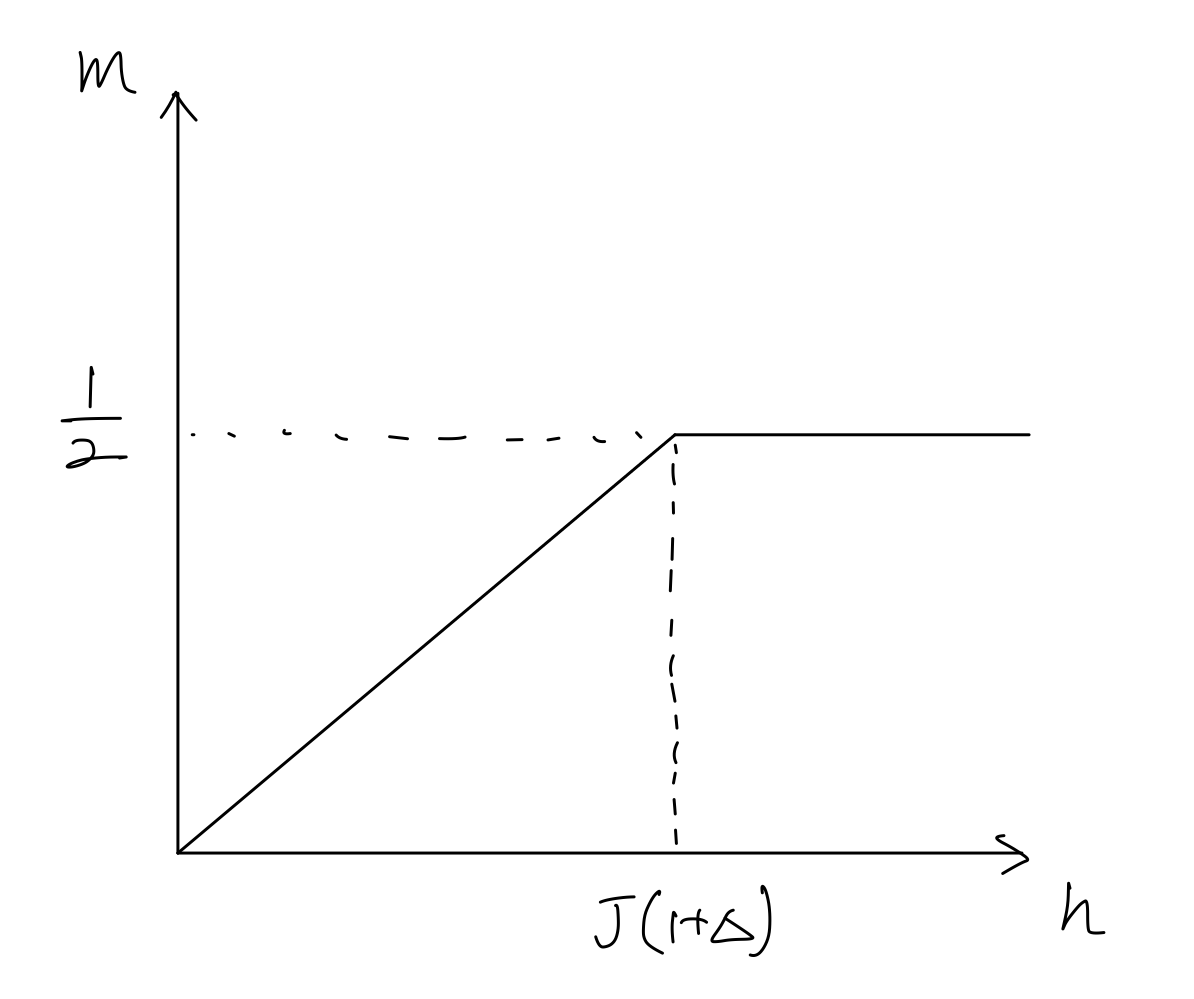
\includegraphics[width=6cm]{jika_1.png}
  \fgcaption{磁化過程}
\end{center}
\subsection*{(d)}
N\'{e}el状態におけるエネルギー期待値を計算する.
まず$S_j^+S_{j+1^-}$の期待値は, $j$が偶数のとき
\end{document}